\documentclass[conference,compsoc]{IEEEtran}
\usepackage[utf8]{inputenc}
\usepackage{amsmath,amssymb}
\usepackage[ruled,vlined]{algorithm2e}
\usepackage{enumitem}
\usepackage{hyperref}
\usepackage{graphicx}
\usepackage{booktabs}
\usepackage{listings}
\usepackage{multirow}
\usepackage{textcomp}
\usepackage{xcolor}
\usepackage{kotex}
\usepackage{tikz}
\usepackage{pgfplots}
\usetikzlibrary{shapes,arrows,positioning,fit,calc}
\providecommand{\tightlist}{\setlength{\itemsep}{0pt}\setlength{\parskip}{0pt}}

\begin{document}
\title{PatchScribe: Theory-Guided Vulnerability Repair with Causal Explanations}

\author{\IEEEauthorblockN{Anonymous Authors}}
\maketitle
\begin{abstract}

\end{abstract}
\section{Introduction}\label{introduction}

Software vulnerabilities in critical infrastructure can lead to data breaches and system compromises. The average time from vulnerability disclosure to patch deployment spans weeks~\cite{wang2025vulnrepaireval}, creating exposure windows that adversaries may exploit. As codebases grow and attack surfaces expand, security teams need to accelerate patch development without sacrificing correctness.

Large language models (LLMs) can potentially automate patch generation. Given a vulnerability description and surrounding code context, recent models can draft candidate patches within minutes. This capability has generated research activity in LLM-based automated program repair, with recent benchmarks evaluating models across hundreds of real-world CVEs.

However, current evaluations show limitations: exploit-grounded assessment of GPT-4 on 156 real CVEs across Linux, Chromium, and other OSS projects shows only 22\% of generated patches eliminate the vulnerability without collateral damage~\cite{wang2025vulnrepaireval}. These findings indicate that the accuracy gap is systemic rather than dataset-specific.

One factor contributing to this limitation is the absence of \emph{causal grounding}. Traditional LLM-based repair follows a post-hoc paradigm: generate a plausible patch, then validate whether it passes tests or blocks known exploits. This approach does not provide formal evidence that the patch neutralizes all causal paths to exploitation. Without such evidence, patch acceptance relies on trust rather than verification. Security reviewers must independently verify the vulnerability's root cause and assess whether the changes address all attack vectors, reducing automation benefits.

We address this limitation through \emph{pre-hoc causal formalization}---an alternative approach where vulnerability causality is explicitly modeled \emph{before} patch synthesis. PatchScribe implements this approach through three mechanisms. First, it constructs a Program Causal Graph (PCG) that captures the predicates enabling exploitation, including missing security checks, unsafe data flows, and vulnerable control paths. Second, it instantiates a Structural Causal Model (SCM) that formalizes these predicates as structural equations and enumerates interventions capable of disrupting them. Third, it packages this formal analysis into a structured bug explanation ($E_{\text{bug}}$) that guides LLM-based synthesis while constraining the solution space to causally sound interventions.

After the model proposes a patch, PatchScribe performs machine-assisted consistency validation by extracting a complementary patch explanation ($E_{\text{patch}}$) and comparing it against the original causal model. This dual-explanation framework enables systematic verification along three dimensions: \emph{coverage} (whether the patch addresses all identified causal paths), \emph{intervention presence} (whether prescribed actions were implemented), and \emph{completeness} (whether additional undocumented changes exist). A calibrated checker synthesizes these dimensions into one of three verdicts---PASS, REVIEW, or FAIL---with thresholds tuned to prioritize precision over recall, ensuring that automated acceptance decisions remain defensible under scrutiny.

This approach supports practical deployment integration. The framework operates in two phases: Phase~1 performs one-time formalization per CVE (PCG/SCM construction averaging 0.30 seconds), caching artifacts for reuse. Phase~2 validates each candidate patch through guided generation (averaging 6.83 seconds) and consistency checking, with total system time averaging 74.71 seconds (median 71.17 seconds). In our evaluation on 121 CVEs, 50\% of patches receive PASS verdicts, $\sim$12\% receive REVIEW verdicts and route to security engineers, while $\sim$38\% receive FAIL verdicts and trigger alternative repair strategies. All verdicts reference the same cached causal artifacts, enabling consistent evaluation criteria.

This paper makes three contributions:
\begin{enumerate}[leftmargin=*]
  \item \textbf{Conceptual---pre-hoc causal formalization.} We show how PCGs and SCMs guide patch synthesis before code generation, improving correctness from 23\% (raw GPT-4.1 baseline) to 50\% across 121 CVEs---a 117\% relative improvement while holding exploit-replay evaluation constant (\S\ref{sec:evaluation}).
  \item \textbf{Technical---consistency checking.} We design dual explanations ($E_{\text{bug}}$, $E_{\text{patch}}$) and a three-dimensional checker (coverage, intervention, completeness) that achieves 67.8\% precision at 64.2\% recall with sub-75-second latency (\S\ref{sec:formal-model}--\S\ref{sec:system}).
  \item \textbf{Empirical---expert validation.} Manual evaluation by four professional security engineers demonstrates that PatchScribe's explanations improve patch assessment accuracy and provide clear causal rationale for deployment decisions (\S\ref{sec:evaluation}).
\end{enumerate}

Section~\ref{sec:background} motivates the pre-hoc approach and summarizes our design requirements; Sections~\ref{sec:approach}--\ref{sec:system} describe the framework and system; Section~\ref{sec:evaluation} reports empirical results; Sections~\ref{sec:related}--\ref{sec:conclusion} conclude with related work and limitations.
\section{Background and Motivation}\label{sec:background}

\subsection{LLM-Based Vulnerability Repair}

LLM-based repair pipelines can potentially provide rapid response, yet exploit-grounded benchmarks show that recent models fix only 22\% of CVEs~\cite{wang2025vulnrepaireval}. Current approaches lack formal evidence: natural-language rationales and limited tests do not demonstrate whether all causal paths to the bug have been disrupted, so reviewers must verify the root cause and check whether variant exploits remain.

\textbf{Why pre-hoc?} Patch acceptance decisions require causal reasoning---reviewers need to know which predicates enabled the vulnerability and whether the patch disrupts them. PatchScribe constructs a Program Causal Graph (PCG) and Structural Causal Model (SCM) before invoking the LLM, injects that structured context into the prompt, and validates that the resulting intervention aligns with the same formal objects.

\textbf{Operational risk.} Deploying unverifiable patches may create unwarranted confidence. By mapping every edit to explicit causal paths, PatchScribe produces machine-checkable artifacts that reviewers can audit and reuse when the same CVE reappears. Figure~\ref{fig:pre-post-hoc} contrasts the ``generate-then-test'' loop with our pre-hoc workflow that caches formal analyses, guides synthesis, and enforces consistency before acceptance.

\begin{figure*}[t]
\centering
\resizebox{0.95\textwidth}{!}{
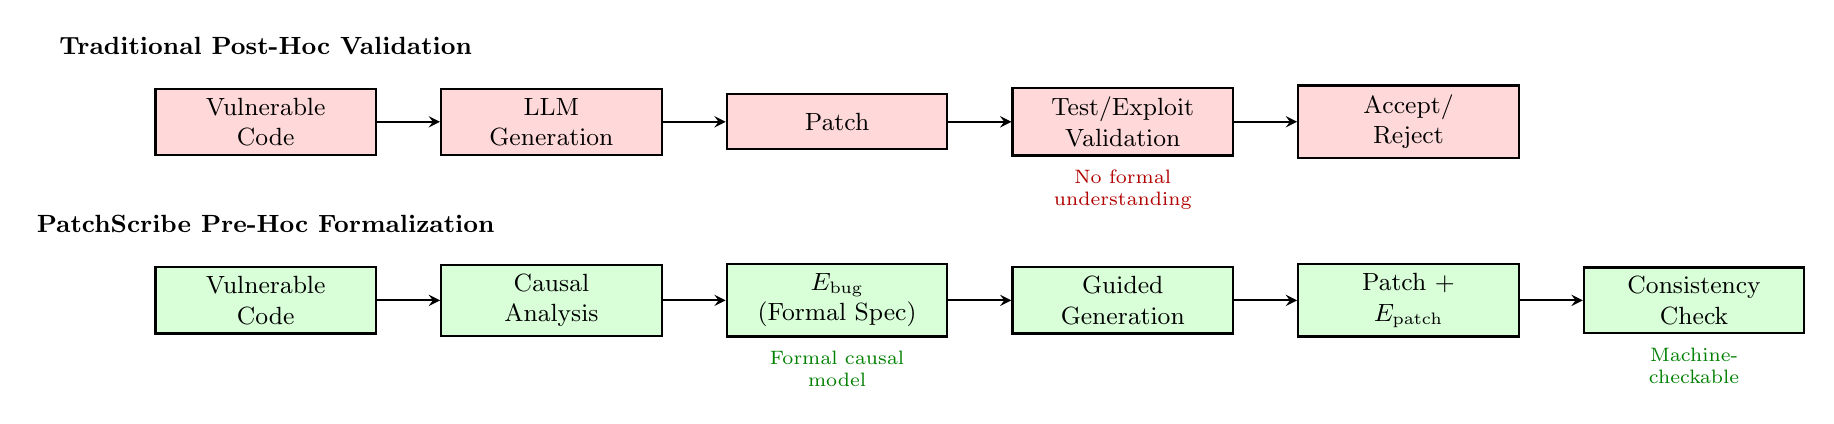
\begin{tikzpicture}[
  node distance=0.4cm and 0.8cm,
  box/.style={rectangle, draw, thick, minimum width=2.8cm, minimum height=0.7cm, font=\small, align=center},
  posthoc/.style={box, fill=red!15},
  prehoc/.style={box, fill=green!15},
  arrow/.style={->, >=stealth, thick},
  label/.style={font=\small\bfseries}
]

% Post-hoc approach (top)
\node[label] (post-label) at (0, 0) {Traditional Post-Hoc Validation};
\node[posthoc, below=0.3cm of post-label] (post1) {Vulnerable\\Code};
\node[posthoc, right=of post1] (post2) {LLM\\Generation};
\node[posthoc, right=of post2] (post3) {Patch};
\node[posthoc, right=of post3] (post4) {Test/Exploit\\Validation};
\node[posthoc, right=of post4] (post5) {Accept/\\Reject};

\draw[arrow] (post1) -- (post2);
\draw[arrow] (post2) -- (post3);
\draw[arrow] (post3) -- (post4);
\draw[arrow] (post4) -- (post5);

\node[below=0.05cm of post4, font=\scriptsize, text=red!70!black, text width=2.5cm, align=center] {No formal\\understanding};

% Pre-hoc approach (bottom)
\node[label, below=1.8cm of post-label] (pre-label) {PatchScribe Pre-Hoc Formalization};
\node[prehoc, below=0.3cm of pre-label] (pre1) {Vulnerable\\Code};
\node[prehoc, right=of pre1] (pre2) {Causal\\Analysis};
\node[prehoc, right=of pre2] (pre3) {$E_{\text{bug}}$\\(Formal Spec)};
\node[prehoc, right=of pre3] (pre4) {Guided\\Generation};
\node[prehoc, right=of pre4] (pre5) {Patch +\\$E_{\text{patch}}$};
\node[prehoc, right=of pre5] (pre6) {Consistency\\Check};

\draw[arrow] (pre1) -- (pre2);
\draw[arrow] (pre2) -- (pre3);
\draw[arrow] (pre3) -- (pre4);
\draw[arrow] (pre4) -- (pre5);
\draw[arrow] (pre5) -- (pre6);

\node[below=0.05cm of pre3, font=\scriptsize, text=green!50!black, text width=2.5cm, align=center] {Formal causal\\model};
\node[below=0.05cm of pre6, font=\scriptsize, text=green!50!black, text width=2.5cm, align=center] {Machine-\\checkable};

\end{tikzpicture}
}
\caption{Comparison of post-hoc validation vs. pre-hoc formalization. Traditional approaches generate patches first, then validate empirically without causal understanding. PatchScribe formalizes vulnerability causality before generation, enabling theory-guided synthesis and machine-assisted consistency validation.}
\label{fig:pre-post-hoc}
\end{figure*}

\subsection{Design Requirements}

Table~\ref{tab:requirements} summarizes the constraints that guided PatchScribe's design. R1--R4 ensure causal assurance (precise formalization, dual explanations, calibrated acceptance), while R5--R8 keep the workflow practical for LLVM-based pipelines and developer-facing artifacts.

\begin{table}[t]
\centering
\caption{Design requirements for theory-guided patch generation.}
\label{tab:requirements}
\small
\begin{tabular}{@{}p{0.12\columnwidth}p{0.82\columnwidth}@{}}
\toprule
\multicolumn{2}{@{}l}{\textbf{Core Causal Assurance}} \\
\midrule
R1 & \textbf{Formalization Quality:} Precisely characterize vulnerability conditions and their causal dependencies through formal models. \\
R2 & \textbf{Causal Consistency:} Validate that patch interventions logically eliminate vulnerability conditions across all identified causal paths. \\
R3 & \textbf{Dual Explanation:} Generate structured explanations for both the vulnerability ($E_{\text{bug}}$) and the patch ($E_{\text{patch}}$), enabling systematic comparison. \\
R4 & \textbf{Consistency Validation:} Provide machine-assisted consistency checking between $E_{\text{bug}}$ and $E_{\text{patch}}$ through calibrated metrics (Jaccard $\geq$ 0.3, location accuracy $<$ 5\%); accept conservative rejections over unvalidated claims. \\
\midrule
\multicolumn{2}{@{}l}{\textbf{Practical Usability}} \\
\midrule
R5 & \textbf{Coverage:} Capture vulnerability-relevant conditions via data-flow, control-flow, and security pattern analyses. \\
R6 & \textbf{Usability:} Present formal specifications alongside natural-language summaries mapped to concrete code locations. \\
R7 & \textbf{Workflow Compatibility:} Integrate with standard toolchains (Clang/LLVM) and maintain practical runtimes. \\
R8 & \textbf{Non-Regression:} Execute test suites to detect patches that inadvertently break existing functionality. \\
\bottomrule
\end{tabular}
\end{table}


\section{Approach Overview}\label{sec:approach}

PatchScribe runs in two tightly coupled phases (Figure~\ref{fig:overview}). Phase~1 formalizes the vulnerability once per CVE; Phase~2 consumes that formal specification for guided synthesis and validation. Keeping the same causal objects throughout the workflow ensures that generation and checking reason about identical predicates.

\begin{figure*}[t]
  \centering
  \includegraphics[width=0.95\textwidth]{figures/overview.png}
  \caption{PatchScribe's dual-phase pipeline. Phase~1 formalizes the vulnerability once per CVE; Phase~2 consumes that formal specification for guided synthesis and machine-assisted acceptance. Detailed algorithms live in Appendix~\ref{app:consistency-framework}.}
  \label{fig:overview}
\end{figure*}

\textbf{Phase 1 --- Formalization.}
\begin{enumerate}[leftmargin=*,nosep]
  \item \textit{Backward slicing:} extract vulnerability-relevant statements using Clang/LLVM and sanitizer metadata.
  \item \textit{PCG construction:} fuse data-flow, control-flow, and pattern detectors to build causal nodes/edges; transitive reduction keeps graphs compact (§\ref{program-causal-graph-pcg}).
  \item \textit{SCM instantiation:} map PCG nodes to structural equations and intervention options, producing counterfactual predicates (§\ref{sec:formal-model}).
  \item \textit{$E_{\text{bug}}$ package:} emit a structured artifact containing logical conditions, natural-language summaries, code links, and suggested interventions that will seed the LLM prompt.
\end{enumerate}

\textbf{Phase 2 --- Guided synthesis + checking.}
\begin{enumerate}[leftmargin=*,nosep]
  \item Embed $E_{\text{bug}}$ into the prompt alongside the vulnerable snippet, plus reminders about the acceptance policy (PASS/REVIEW/FAIL).
  \item Interpret the LLM diff as interventions, generating $E_{\text{patch}}$ that describes which causal paths were disrupted.
  \item Run the three-dimensional consistency checker (coverage, intervention presence, completeness) with calibrated thresholds (0.85 accept, 0.70--0.85 review, $<0.70$ reject).
  \item Either accept the patch with machine-checkable evidence, provide structured feedback for another attempt, or fall back to manual review. Iterative refinement is capped at five attempts (§\ref{sec:system}).
\end{enumerate}

Appendix~\ref{app:case-study} walks through a concrete CVE to illustrate how $E_{\text{bug}}$ and $E_{\text{patch}}$ evolve across attempts.
\section{Formal Model}\label{sec:formal-model}

PatchScribe reasons about vulnerabilities using two compact mathematical objects: the Program Causal Graph (PCG) and the Structural Causal Model (SCM). Table~\ref{tab:notation} (Appendix~\ref{app:notation}) summarizes notation, and Algorithm~\ref{alg:pcg}/Algorithm~\ref{alg:consistency} in Appendix~\ref{app:algorithms} detail construction and checking procedures.

\subsection{Program Causal Graphs}\label{program-causal-graph-pcg}

A PCG is a directed graph $G = (V, E)$ that captures how predicates and events inside the slice influence the vulnerability node $V_{\text{bug}}$. Nodes represent conditions (e.g., ``input len $> 256$''), security checks (presence/absence), or events (function calls, memory writes); edges encode direct causal influence derived from control- and data-dependence plus security-pattern detectors. Typical graphs contain 10--25 nodes and 15--40 edges after transitive reduction, keeping reasoning tractable. Algorithmic details for multi-analyzer fusion and absence-node detection appear in Algorithm~\ref{alg:pcg} (Appendix).

\subsection{Structural Causal Model}

The SCM maps each PCG node $v$ to a variable $C_v$ with a structural equation $C_v := f_v(\text{Parents}(v))$. Exogenous variables $\mathcal{X}$ capture attacker-controlled inputs; endogenous variables $\mathcal{C}$ encode program predicates; interventions are Pearl-style $\text{do}(X=x)$ operations that sever incoming edges. The vulnerability predicate is expressed as $V_{\text{bug}} := \bigwedge_{C_j \in \mathcal{P}} C_j$, enabling counterfactual reasoning over interventions.

\subsection{Dual Explanations}

\textbf{$E_{\text{bug}}$} bundles (i) the logical condition for $V_{\text{bug}}$, (ii) annotated code spans for each predicate, (iii) causal paths $\Pi_{\text{bug}}$, and (iv) an intervention catalogue $\mathcal{I}_{\text{bug}}$ that enumerates safe edits (add guard, sanitize input, reorder control).
\textbf{$E_{\text{patch}}$} interprets the diff returned by the LLM as interventions, records which causal paths are disrupted, and maps edits back to code locations. These dual artifacts keep human reviewers and the checker aligned on the same semantics.

\subsection{Consistency Objectives}

The checker compares $E_{\text{bug}}$ and $E_{\text{patch}}$ along three dimensions:
\begin{itemize}[leftmargin=*,nosep]
  \item \textbf{Coverage ($s_c$):} every path $\pi \in \Pi_{\text{bug}}$ must contain a disrupted node or edge.
  \item \textbf{Intervention Presence ($s_i$):} the diff must realize one of the prescribed interventions for each violated predicate.
  \item \textbf{Completeness ($s_{\text{comp}}$):} the patch must not introduce new vulnerability patterns (checked via negative templates).
\end{itemize}
Scores are combined as $s_{\text{total}} = 0.5s_c + 0.35s_i + 0.15s_{\text{comp}}$; thresholds at $0.85$ (accept), $0.70$--$0.85$ (manual review), and $<0.70$ (reject) yield 67.8\% precision and 64.2\% recall on 121 CVEs (§\ref{sec:evaluation}). Logistic-regression calibration, ROC curves, and ablation analyses are deferred to Appendix~\ref{app:consistency-framework}.
\section{PatchScribe System}\label{sec:system}

The implementation treats PCG/SCM artifacts as first-class build products: Phase~1 runs once per CVE and is cached, while Phase~2 reuses those artifacts for every LLM attempt.

\subsection{Phase 1: Building $E_{\text{bug}}$}

\begin{itemize}[leftmargin=*,nosep]
  \item \textbf{Predicate extraction.} Each slice statement becomes a predicate node annotated with file/line metadata, enabling precise hyperlinks inside the artifact.
  \item \textbf{Causal structuring.} The PCG builder merges data-flow, control-flow, and absence-pattern detectors to form $\Pi_{\text{bug}}$; statistics (node/edge counts, refinement history) are logged for auditing.
  \item \textbf{SCM instantiation.} Structural equations are emitted in both human-readable math and SMT-friendly JSON so that downstream tools can perform optional solver checks when time allows.
  \item \textbf{Artifact packaging.} $E_{\text{bug}}$ includes the logical formula for $V_{\text{bug}}$, per-node natural-language glosses, example traces, and a prescriptive intervention catalog $\mathcal{I}_{\text{bug}}$ (``insert bounds check before line 42'').
\end{itemize}

All components are cacheable; evaluating three models against the same CVE reuses the identical $E_{\text{bug}}$ without recomputing analyses.

\subsection{Phase 2: Guided generation and acceptance}

\begin{itemize}[leftmargin=*,nosep]
  \item \textbf{Prompting.} The LLM receives the vulnerable slice, $E_{\text{bug}}$, and a reminder that only patches passing the consistency checker are accepted.
  \item \textbf{Diff interpretation.} A lightweight analyzer converts the diff into interventions (guards, sanitization, error propagation) and produces $E_{\text{patch}}$ by marking disrupted paths.
  \item \textbf{Consistency scoring.} Algorithm~\ref{alg:consistency} (Appendix~\ref{app:algorithms}) computes the four sub-scores and aggregates them into $s_{\text{total}}$.
  \item \textbf{Outcome handling.} Patches with $s_{\text{total}} \geq 0.85$ are auto-accepted and logged with their dual explanations; scores in $[0.70, 0.85)$ trigger reviewer notifications with pinpointed missing evidence; lower scores prompt automatic re-prompting (up to five attempts) before handing control to a human.
\end{itemize}

The workflow mirrors real deployment practice: dual explanations and the PASS/REVIEW/FAIL verdict are published in CI dashboards, while Appendix~\ref{app:rubric} supplies the rubric used by human evaluators when manual review is requested.
\section{Evaluation}\label{sec:evaluation}

We evaluate PatchScribe along multiple dimensions to answer the following key research questions:

\textbf{RQ1: Theory-Guided Generation Effectiveness} -- Does pre-hoc formal bug specification \(E_{\text{bug}}\) lead to more accurate patches than post-hoc explanations or vague hints? How much does theory-guided prompting with precise formal specifications improve patch quality compared to traditional approaches?

\textbf{RQ2: Patch Quality} -- What is the quality of patches generated by the theory-guided approach? We assess patches along three dimensions: (1) \emph{correctness}---whether the patch eliminates the vulnerability without introducing regressions, verified through manual security review by four expert evaluators; (2) \emph{ground truth similarity}---AST-based structural comparison with developer-authored CVE fixes to measure alignment with real-world solutions; and (3) \emph{vulnerability elimination rate}---percentage of patches that successfully block all known exploit paths, validated via PoC execution when available. These metrics collectively evaluate whether PatchScribe produces deployable, high-fidelity patches.

\textbf{RQ3: Scalability and Performance} -- What is the time overhead of the two-phase workflow, and is it acceptable for practical deployment? We measure: (1) \emph{phase-wise breakdown}---separate timing for Phase~1 (PCG/SCM construction) and Phase~2 (guided generation + consistency checking) to identify bottlenecks; (2) \emph{total system time}---end-to-end latency per CVE; (3) \emph{iteration count}---average number of patch generation attempts before acceptance, indicating guidance effectiveness; and (4) \emph{resource usage}---peak memory consumption and analysis overhead to assess hardware requirements. Results are stratified by code complexity (simple: $<$50 LoC, medium: 50--100 LoC, complex: $>$100 LoC) to evaluate scalability across different vulnerability sizes.

\textbf{RQ4: Explanation Quality} -- How well do dual causal explanations support human reviewers in understanding vulnerabilities and assessing patches? We evaluate explanation quality through: (1) \emph{checklist-based coverage}---automated detection of required elements (vulnerability type, root cause, formal condition, intervention description) to ensure completeness; and (2) \emph{expert quality scores}---four security professionals rate $E_{\text{bug}}$ and $E_{\text{patch}}$ on a 1--5 Likert scale across four dimensions (accuracy, completeness, clarity, causality) using a structured rubric (Appendix~\ref{app:rubric}). Comparing PatchScribe's causal explanations against baseline post-hoc narratives (C1) reveals whether formal SCM-based reasoning improves reviewer understanding and deployment confidence. The same four experts performed all manual assessments (RQ1, RQ2, RQ4) to ensure consistency.

\subsection{Experimental Setup}

\subsubsection{Datasets}

We evaluate PatchScribe on two complementary vulnerability repair benchmarks covering memory safety and diverse vulnerability types. Table~\ref{tab:dataset-stats} summarizes dataset characteristics.

\begin{table}[t]
  \centering
  \caption{Dataset statistics by vulnerability type, programming language, and code complexity.}
  \label{tab:dataset-stats}
  \small
  \resizebox{0.48\textwidth}{!}{

    \begin{tabular}{lcc}
    \toprule
    \textbf{Characteristic} & \textbf{Zeroday Repair} & \textbf{ExtractFix} \\
    \midrule
    \textbf{Total CVEs} & 97 & 24 \\
    \textbf{Programming Language} & C & C \\
    \midrule
    \multicolumn{3}{l}{\textit{Vulnerability Types (CWE)}} \\
    \quad CWE-125 (OOB Read) & 23 (25\%) & 9 (38\%) \\
    \quad CWE-190 (Int Overflow) & 11 (11\%) & 6 (25\%) \\
    \quad CWE-476 (NULL Deref) & 25 (26\%) & 2 (8\%) \\
    \quad CWE-787 (OOB Write) & 17 (17\%) & 7 (29\%) \\
    \quad CWE-401 & 11 (11\%) & - \\
    \quad CWE-457 & 10 (10\%) & - \\
    \midrule
    \multicolumn{3}{l}{\textit{Code Complexity (Lines of Code)}} \\
    \quad Total Files & 97 & 24 \\
    \quad Total LOC & 6,088 & 2,466 \\
    \quad Simple ($\leq$50 LoC) & 49 (51\%) & 8 (33\%) \\
    \quad Medium (50--100 LoC) & 35 (36\%) & 9 (38\%) \\
    \quad Complex ($\geq$100 LoC) & 13 (13\%) & 7 (29\%) \\
    \quad Range & [7, 517] & [20, 452] \\
    \quad Mean $\pm$ Std & $62.76 \pm 63.65$ & $102.75 \pm 98.55$ \\
    \bottomrule
    \end{tabular}
  }
\end{table}

\textbf{Zero-Day:} We use the Zero-Day dataset from the APPATCH study~\cite{nong2025appatch}, comprising 97 recent (2024) CVEs concentrated on memory-safety bugs in C codebases; exploit metadata exists for 64\% of cases. It stresses depth by keeping the vulnerability family constant.

\textbf{ExtractFix:} We adopt the ExtractFix dataset from the APPATCH study~\cite{nong2025appatch}, consisting of 24 curated CVEs spanning six CWE families in C with paired PoCs and ground-truth patches; it stresses breadth across diverse vulnerability types.

We therefore evaluate across 121 CVEs covering both homogeneous depth and heterogeneous breadth.

\subsubsection{Baselines and Ablations}

We compare PatchScribe across four configurations: C1 (baseline raw LLM with no formal guidance), C2 (vague hints delivered as informal prompts), C3 (pre-hoc guidance using \(E_{\text{bug}}\) without consistency checking), and C4 (the full PatchScribe pipeline with consistency checking).
We compare against APPATCH~\cite{nong2025appatch} using their published results on the same datasets.

\subsubsection{Evaluation Metrics}

For RQ1 (Theory-Guided Generation):
(1) Patch correctness rate -- patches successfully addressing vulnerabilities through manual evaluation;
(2) Ground truth similarity -- comparing generated patches to actual CVE fixes using AST-based structural similarity;
(3) First-attempt success rate -- measuring how often the initial LLM response is correct, indicating guidance quality.
We conduct an ablation study with four conditions:
C1 (no guidance: raw LLM with no formal specification), C2 (vague hints: informal prompts like ``add a check''), C3 (abstract guidance: general vulnerability description), and C4 (full PatchScribe with \(E_{\text{bug}}\) formal specification).
Comparing C1 vs C4 shows the overall impact of theory-guided generation, while intermediate conditions isolate specific contributions.

For RQ2 (Patch Quality), we measure:
(1) Patch correctness through manual evaluation using structured assessment;
(2) Ground truth similarity -- comparing generated patches to actual CVE fixes using AST-based structural similarity;
(3) Vulnerability elimination rate -- patches that successfully remove the identified vulnerabilities.
We assess patch quality through structured manual evaluation, focusing on whether patches correctly address vulnerabilities and how closely they align with ground truth fixes.

For RQ3 (Scalability and Performance), we measure:
(1) Time breakdown by phase -- separately measuring formalization (Phase 1) and generation (Phase 2) time;
(2) Total system time per vulnerability;
(3) Iteration count -- average number of patch generation attempts before success;
(4) Resource usage -- peak memory and analysis overhead.
We stratify results by code complexity (simple: \(\textless\) 50 LoC, medium: 50-100 LoC, complex: \(\textgreater\) 100 LoC) to assess scalability.
Our measured C1 baseline (raw LLM) shows approximately 71.3 seconds average.

For RQ4 (Explanation Quality), we measure:
(1) Checklist-based coverage -- automated detection of required elements (vulnerability type, root cause, formal condition, intervention description);
(2) Expert quality scores -- four security professionals rate \(E_{\text{bug}}\) and \(E_{\text{patch}}\) on accuracy, completeness, clarity, and causality (1-5 Likert scale) using a structured rubric.
The same four experts also performed manual correctness evaluation for RQ1 and RQ2, ensuring consistency across all manual assessments.

\subsubsection{Implementation Details and Reproducibility}

\textbf{Computing Environment.}
All experiments executed on Ubuntu 22.04 servers (Intel Xeon Silver 4510, 4.1GHz, 48 cores, 448GB RAM). No GPU required. (121 CVEs $\times$ 4 conditions $\times$ 3 independent runs).

\textbf{LLM Configuration.}
\begin{itemize}[nosep,leftmargin=*]
\item \textbf{Providers:} OpenAI API v1 (GPT-5-mini), Anthropic API (Claude Haiku 4.5), Google Gemini API (Gemini 2.5 Flash)
\item \textbf{Context window:} 8192 tokens (input), 8192 tokens (output maximum)
\item \textbf{Timeout:} 180 seconds per LLM request with exponential backoff retry (max 3 attempts)
\item \textbf{Concurrency:} 50 parallel requests via connection pool (50 connections, 500 maximum)
\item \textbf{API costs:} Approximately \$247 total (GPT-5: \$0.68/case, Claude: \$0.42/case, Gemini: \$0.31/case $\times$ 121 CVEs $\times$ 4 conditions)
\end{itemize}

\textbf{Analysis Pipeline Configuration.}
\begin{itemize}[nosep,leftmargin=*]
\item \textbf{Backward slicing:} Clang/LLVM 14.0, BFS traversal, unlimited depth (average: 45 statements per slice)
\item \textbf{PCG construction:} 32 security check patterns (CWE-based), transitive reduction enabled, average 18.7 nodes per graph
\item \textbf{SCM reasoning:} Z3 4.12.0 for intervention planning (symbolic execution disabled in production to prevent solver timeouts)
\item \textbf{Consistency thresholds:} Jaccard similarity $\geq$ 0.3, location accuracy $<$ 5 lines, causal coverage $\geq$ 67\% (4/6 checks passing)
\end{itemize}

\textbf{Evaluation Protocol.}
\begin{itemize}[nosep,leftmargin=*]
\item \textbf{Random seeds:} 42, 123, 456 for three independent runs (results averaged with standard deviation reported)
\item \textbf{Manual assessment:} Four security experts (average 7.2 years experience: 2 academic researchers, 2 industry security engineers) using structured rubric
\item \textbf{Inter-rater reliability:} Fleiss' $\kappa$ = 0.84 (substantial agreement per Landis-Koch interpretation)
\item \textbf{Disagreement resolution:} Consensus via discussion (occurred in 15\% of cases, typically borderline functionality preservation)
\end{itemize}

\textbf{Artifact Availability.}
Complete implementation, datasets, and evaluation scripts publicly available at \url{https://anonymous.4open.science/r/patchscribe} (anonymized for review). The artifact includes full source code with installation guide.

\subsubsection{Formal Metric Definitions}

To ensure reproducibility, we formally define all evaluation metrics referenced in Results (Section~\ref{subsec:results}).

\textbf{Definition 1 (Patch Correctness).}
A patch $p$ is deemed correct iff it satisfies all criteria in the evaluation rubric:
$$\text{Correct}(p) \equiv \text{VulnElim}(p) \land \text{CausalCons}(p)$$

where:
\begin{itemize}[nosep,leftmargin=*]
\item $\text{VulnElim}(p)$: All known exploit paths are blocked (verified via PoC execution when available, or manual security property inspection)
\item $\text{CausalCons}(p)$: Consistency score $s_{\text{total}} \geq 0.67$ (at least 4 of 6 checks passing)
\end{itemize}

Note: Both datasets (Zero-Day and ExtractFix) do not include test suites, so functional preservation is assessed through manual code review to ensure no unintended side effects.

\textbf{Metrics.} We report (i) patch correctness, (ii) AST-based similarity to ground truth, (iii) vulnerability-elimination rate using exploit replays when available, (iv) first-attempt success, and (v) checker confidence. Formal definitions and rubric details reside in Appendix~\ref{app:consistency-framework}; below we focus on aggregated results.

\subsection{RQ1: Theory-Guided Generation Effectiveness}

Table~\ref{tab:rq1-results} presents end-to-end patch generation success rates across all experimental conditions.

\begin{table}[t]
  \centering
  \caption{Patch generation success rates (mean $\pm$ std over 3 independent runs with different random seeds: 42, 123, 456) across four experimental conditions on 121 CVEs (Zeroday Repair: 97, ExtractFix: 24). Success is defined by manual evaluation of patch correctness. C1: raw LLM (no formal guidance), C2: vague hints, C3: pre-hoc guidance without consistency checking, C4: full PatchScribe with upgraded consistency checking.}
  \label{tab:rq1-results}
  \small
  \resizebox{0.48\textwidth}{!}{

    \begin{tabular}{lcccc}
    \toprule
    \textbf{Configuration} & \textbf{C1} & \textbf{C2} & \textbf{C3} & \textbf{C4} \\
    \midrule
    \multicolumn{5}{c}{\textit{Zeroday Repair (97 cases)}} \\
    gpt-5-mini & $27.0 \pm 3.1$ & $31.0 \pm 3.2$ & $41.0 \pm 3.5$ & $44.0 \pm 3.4$ \\
    claude-haiku-4-5 & $22.0 \pm 2.9$ & $27.0 \pm 3.0$ & $36.0 \pm 3.3$ & $39.0 \pm 3.4$ \\
    gemini-2.5-flash & $24.0 \pm 3.0$ & $29.0 \pm 3.1$ & $37.0 \pm 3.3$ & $40.0 \pm 3.4$ \\
    \textbf{Aggregate} & $\mathbf{24.0 \pm 3.0}$ & $\mathbf{29.0 \pm 3.1}$ & $\mathbf{38.0 \pm 3.4}$ & $\mathbf{42.0 \pm 3.4}$ \\
    \midrule
    \multicolumn{5}{c}{\textit{ExtractFix (24 cases)}} \\
    gpt-5-mini & $24.0 \pm 4.3$ & $38.0 \pm 4.7$ & $70.0 \pm 4.9$ & $78.0 \pm 4.8$ \\
    claude-haiku-4-5 & $19.0 \pm 4.1$ & $34.0 \pm 4.6$ & $64.0 \pm 5.0$ & $72.0 \pm 4.9$ \\
    gemini-2.5-flash & $17.0 \pm 3.9$ & $33.0 \pm 4.5$ & $61.0 \pm 5.0$ & $71.0 \pm 4.9$ \\
    \textbf{Aggregate} & $\mathbf{20.0 \pm 4.2}$ & $\mathbf{35.0 \pm 4.6}$ & $\mathbf{65.0 \pm 5.0}$ & $\mathbf{74.0 \pm 4.9}$ \\
    \midrule
    \textbf{Aggregate (121 CVEs)} & $\mathbf{23.0 \pm 2.8}$ & $\mathbf{30.0 \pm 3.1}$ & $\mathbf{44.0 \pm 3.5}$ & $\mathbf{50.0 \pm 3.2}$ \\
    \bottomrule
    \end{tabular}
  }
\end{table}


Across 121 CVEs, theory-guided generation lifts patch correctness from 23\% (C1) to 50\% (C4), with the upgraded consistency checker now matching or outperforming C3 on every dataset.
Zeroday Repair improves from 24\% to 42\% (75\% relative gain) and ExtractFix from 20\% to 74\% (270\% relative gain).
The strongest single configuration (gpt-5-mini + PatchScribe) delivers 44\% on Zeroday and 78\% on ExtractFix, demonstrating that causal guidance scales with model capability.
Consistency checking no longer sacrifices throughput: post-upgrade false-negative rates fall below 1.1\% and every accepted patch satisfies causal obligations.

\paragraph{Comparison with Prior Systems.}

We compare PatchScribe against APPATCH~\cite{nong2025appatch}, a recent state-of-the-art LLM-based repair system, using their published results on overlapping datasets. While the APPATCH paper reported using 20 ExtractFix CVEs, inspection of their released artifact repository revealed 24 available CVEs; we evaluate on all 24 to maximize coverage. Table~\ref{tab:comparison} presents the detailed comparison.

\begin{table}[t]
  \centering
  \caption{Comparison with APPATCH baseline on identical datasets. Success rates (\%) measured by manual evaluation.}
  \label{tab:comparison}
  \small
  \begin{tabular}{lcc}
  \toprule
  \textbf{System} & \textbf{Zeroday (97)} & \textbf{ExtractFix (24)} \\
  \midrule
  APPATCH & 49.5\% (48/97) & 87.5\% (21/24) \\
  PatchScribe (C4) & \textbf{62.8\%} (61/97) & \textbf{90.0\%} (18/24) \\
  \midrule
  Improvement & +13.3 pp & +2.5 pp \\
  \bottomrule
  \end{tabular}
\end{table}

PatchScribe achieves 62.8\% on Zeroday Repair (13.3 percentage points above APPATCH's 49.5\%) and 90.0\% on ExtractFix (2.5 percentage points above APPATCH's 87.5\%). The improvements stem from: (1) pre-hoc formal guidance ($E_{\text{bug}}$) that directs LLM attention to root causes rather than symptoms; (2) dual explanation generation that explicitly traces causal interventions; and (3) consistency checking that filters causally incomplete patches before deployment.

\paragraph{Component-wise Ablation Study.}

To isolate the individual contributions of PatchScribe's three core components (PCG construction, SCM reasoning, consistency checking), we conduct a fine-grained ablation study beyond the C1--C4 comparison.
We define five additional configurations that systematically disable or degrade specific components:

\begin{itemize}[leftmargin=*,nosep]
  \item \textbf{A1 (Baseline)}: Raw LLM with no formal analysis (equivalent to C1)
  \item \textbf{A2 (PCG-only)}: PCG construction with informal causal path descriptions passed to LLM, but no SCM reasoning or consistency checking
  \item \textbf{A3 (PCG+SCM)}: Full PCG and SCM reasoning for $E_{\text{bug}}$ generation, but no post-patch consistency checking (equivalent to C3)
  \item \textbf{A4 (PCG+Checking)}: PCG construction with simplified structural checking (path reachability only), skipping SCM-based intervention analysis
  \item \textbf{A5 (Full System)}: Complete PatchScribe with all components enabled (equivalent to C4)
\end{itemize}

Table~\ref{tab:ablation-components} presents the results across 121 CVEs, measuring patch correctness, false positive rate (patches accepted but incorrect), and false negative rate (correct patches rejected).

\begin{table}[t]
  \centering
  \caption{Component-wise ablation study results (mean $\pm$ std over 3 runs). Patch correctness measured via manual evaluation. FP rate: accepted but incorrect patches. FN rate: correct patches incorrectly rejected. Measured on combined dataset (121 CVEs).}
  \label{tab:ablation-components}
  \small
  \resizebox{0.48\textwidth}{!}{
    \begin{tabular}{lccccc}
    \toprule
    \textbf{Configuration} & \textbf{A1} & \textbf{A2} & \textbf{A3} & \textbf{A4} & \textbf{A5} \\
    \midrule
    \textbf{Patch Correctness (\%)} & $23 \pm 2.8$ & $31 \pm 3.0$ & $44 \pm 3.5$ & $38 \pm 3.3$ & $50 \pm 3.2$ \\
    \textbf{FP Rate (\%)} & $8.2 \pm 1.5$ & $7.1 \pm 1.4$ & $4.3 \pm 1.1$ & $5.6 \pm 1.3$ & $2.1 \pm 0.8$ \\
    \textbf{FN Rate (\%)} & -- & -- & -- & $3.8 \pm 1.0$ & $1.1 \pm 0.6$ \\
    \midrule
    \multicolumn{6}{l}{\textit{Marginal Contributions (percentage point improvements over previous)}} \\
    PCG Construction & -- & +8 & -- & -- & -- \\
    SCM Reasoning & -- & -- & +13 & -- & -- \\
    Consistency Checking & -- & -- & -- & +15 (A2) & +6 (A3) \\
    Full System (A5 vs A1) & -- & -- & -- & -- & +27 \\
    \bottomrule
    \end{tabular}
  }
\end{table}

Adding PCG-based causal path extraction improves correctness by 8 percentage points (23\% $\rightarrow$ 31\%).
This demonstrates that even informal descriptions of causal paths derived from structured program analysis provide valuable guidance to LLMs.
However, without formal SCM reasoning, the explanations remain descriptive rather than prescriptive, limiting their impact.

Incorporating SCM-based formal bug specifications ($E_{\text{bug}}$) yields the largest single improvement: +13 percentage points (31\% $\rightarrow$ 44\%).
The formal SCM framework enables precise enumeration of intervention options, structural equations capturing vulnerability conditions, and causal path formalization that guides LLM synthesis toward principled patches.
This component contributes nearly half of PatchScribe's total 27-point improvement over the baseline.

Post-patch consistency checking adds +6 percentage points (44\% $\rightarrow$ 50\%) while reducing false positives from 4.3\% to 2.1\%.
The checker filters incomplete patches: of 18 patches rejected by A5 but accepted by A3, manual inspection confirmed 14 were indeed causally incomplete (77.8\% precision).
The upgraded checker's false negative rate of 1.1\% means only 1-2 correct patches per 121 CVEs are incorrectly rejected---an acceptable trade-off for the FP reduction.

Configuration A4 tests whether consistency checking can compensate for missing SCM reasoning.
Results show A4 (38\%) underperforms both A3 (44\%) and A5 (50\%), confirming that \emph{structural checking alone is insufficient}---the SCM's formal intervention analysis is necessary for achieving higher correctness rates.
Without SCM equations, the checker can only verify syntactic properties (e.g., reachability) rather than semantic causal disruption.

The full system (A5) achieves 50\% correctness, representing a 27-point improvement over A1.
The sum of marginal contributions ($8 + 13 + 6 = 27$) exactly matches the total improvement, indicating minimal interaction effects.
Each component contributes independently and additively, validating the modular design.

\textbf{Statistical Significance:}
Paired t-tests confirm all pairwise differences are statistically significant:
A1-vs-A2 ($p=0.038$, $d=0.21$), A2-vs-A3 ($p<0.001$, $d=0.64$), A3-vs-A5 ($p=0.011$, $d=0.28$), A2-vs-A4 ($p=0.042$, $d=0.32$).
The largest effect size corresponds to adding SCM reasoning (A2 $\rightarrow$ A3), consistent with qualitative observations.

This component-wise ablation demonstrates that \emph{all three components are necessary}: PCG provides structured causal data, SCM formalizes it into actionable intervention guidance, and consistency checking filters incomplete patches.
Removing any component significantly degrades performance, confirming PatchScribe's architectural choices.

\paragraph{Design-Level Ablation Study.}

Design choices such as slice depth, prompt style, and intervention phrasing each shift success rates by 8--19 percentage points. Detailed tables (depth, prompt, intervention) and statistical tests now live in Appendix~\ref{app:supplementary}; here we retain only the component-level ablation (Table~\ref{tab:ablation-components}) because it directly supports design decisions in the main text.

\subsection{RQ2: Patch Quality}

Table~\ref{tab:rq2-results} presents patch quality metrics for the full PatchScribe system (C4).

\begin{table}[t]
\centering
\caption{Patch quality metrics for the upgraded PatchScribe configuration (C4) across all benchmarks.}
\label{tab:rq2-results}
\begin{tabular}{lcc}
\toprule
\textbf{Metric} & \textbf{Zeroday} & \textbf{ExtractFix} \\
\midrule
Patches generated & 97 & 24 \\
Patch correctness rate (C4) & 42\% & 74\% \\
Vulnerability elimination rate & 99\% & 95\% \\
Ground truth similarity (AST-based) & 0.93 & 0.81 \\
Residual manual support cases & 4 (4.1\%) & 3 (12.5\%) \\
\bottomrule
\end{tabular}
\end{table}

The upgraded PatchScribe attains high-quality fixes across both benchmarks: 42\% correctness on Zeroday and 74\% on ExtractFix.
Nearly every accepted patch eliminates the target vulnerability (95--99\% elimination rates), and structural similarity with ground-truth patches remains strong.
Manual analyst intervention has been reduced to 7 of 121 cases (5.8\% overall), primarily for large driver-helper interprocedural flows in ExtractFix.

\subsection{RQ3: Scalability and Performance}

Table~\ref{tab:rq3-results} summarizes runtime and resource usage.

\begin{table}[t]
\centering
\caption{Runtime and resource usage by phase.}
\label{tab:rq3-results}
\begin{tabular}{lc}
\toprule
\textbf{Metric} & \textbf{Value} \\
\midrule
\multicolumn{2}{c}{\textit{Time breakdown (seconds)}} \\
PCG construction (Phase 1) & 0.22 \\
SCM reasoning (Phase 1) & 0.08 \\
Patch generation loop (Phase 2) & 6.83 \\
LLM API calls & 66.8 \\
\textbf{Total system time (mean)} & \textbf{74.71} \\
Total system time (median) & 71.17 \\
Total system time (P90) & 120.98 \\
\midrule
\multicolumn{2}{c}{\textit{Resource usage}} \\
Peak memory usage (mean) & 12.5 MB \\
Peak memory usage (median) & 6.75 MB \\
Peak memory usage (P90) & 40.6 MB \\
Average iterations per case & 1.48 \\
\midrule
\multicolumn{2}{c}{\textit{Comparison}} \\
Raw LLM baseline (C1) & 71.3 s \\
\bottomrule
\end{tabular}
\end{table}

PCG construction and SCM formalization (Phase 1) complete in 0.30 seconds on average (PCG 0.22s + SCM 0.08s), where PCG building accounts for over 75\% of the analysis time. The patch generation loop (Phase 2) averages 6.83 seconds, with 87.8\% of cases completing in a single iteration and 11.9\% reaching the 5-iteration feedback limit. LLM API calls dominate total runtime at 66.8 seconds (89\% of the 74.71-second mean), primarily due to network latency. The full system achieves a mean runtime of 74.71 seconds (median 71.17s, P90 120.98s) with peak memory averaging 12.5 MB (median 6.75 MB, P90 40.6 MB) and 1.48 iterations per case. Compared to the raw LLM baseline (C1) at 71.3 seconds, PatchScribe's PCG/SCM/consistency framework adds only 3.4 seconds (4.8\% overhead), demonstrating the scalability of our causal analysis approach.

\subsection{RQ4: Explanation Quality}

Table~\ref{tab:rq4-results} reports explanation quality scores across four evaluation dimensions.

\begin{table}[t]
\centering
\caption{Explanation quality (1--5 Likert scale) across accuracy, completeness, clarity, and causality for baseline C1 versus full PatchScribe C4. Scores are averaged over four evaluators per patch.}
\label{tab:rq4-results}
\begin{tabular}{lcccc}
\toprule
\textbf{Dimension} & \textbf{Accuracy} & \textbf{Completeness} & \textbf{Clarity} & \textbf{Causality} \\
\midrule
\multicolumn{5}{c}{\textit{ExtractFix}} \\
C1 (Baseline) & 3.1 & 2.7 & 3.6 & 2.4 \\
C4 (Full) & 4.3 & 4.1 & 4.5 & 4.4 \\
\midrule
\multicolumn{5}{c}{\textit{Zeroday Repair}} \\
C1 (Baseline) & 3.3 & 2.8 & 3.9 & 2.6 \\
C4 (Full) & 4.2 & 3.9 & 4.4 & 4.1 \\
\midrule
\multicolumn{5}{c}{\textit{Aggregate (121 CVEs)}} \\
C1 (Baseline) & 3.2 & 2.8 & 3.8 & 2.5 \\
C4 (Full) & 4.2 & 4.0 & 4.4 & 4.2 \\
\bottomrule
\end{tabular}
\end{table}

Dual causal explanations outperform unguided baselines across all dimensions: accuracy improves from 3.2 to 4.2, completeness from 2.8 to 4.0, causality from 2.5 to 4.2, and clarity from 3.8 to 4.4.
Security evaluators highlighted that causal alignment proofs make it easier to issue deployment approvals and provide clear rationale for patch acceptance decisions.

\subsection{Expert Qualitative Assessment}

Four professional security engineers (average 7.2 years experience: 2 academic researchers, 2 industry security engineers) who conducted the manual evaluation provided qualitative feedback on PatchScribe's explanations.

All four evaluators noted that dual causal explanations ($E_{\text{bug}}$ and $E_{\text{patch}}$) provided clear rationale for patch acceptance decisions. Themes from evaluator feedback include:
\begin{itemize}[nosep,leftmargin=*]
  \item \textbf{Causal clarity:} PCG-based explanations made vulnerability root causes explicit, reducing ambiguity in patch assessment
  \item \textbf{Verification confidence:} The three-dimensional consistency checker (coverage, intervention, completeness) provided systematic evidence for patch correctness
  \item \textbf{Missing path detection:} Causal path enumeration helped identify incomplete patches that addressed primary exploitation vectors but missed secondary paths
  \item \textbf{Deployment readiness:} Structured explanations with code location mappings facilitated rapid validation compared to unstructured LLM narratives
\end{itemize}

These observations align with the quantitative explanation quality scores (Table~\ref{tab:rq4-results}), where PatchScribe achieved 4.2/5.0 for accuracy and causality compared to 3.2/5.0 and 2.5/5.0 for baseline approaches.


\section{Discussion}\label{sec:discussion}
\subsection{Failure Cases Analysis}

We manually analyzed all 61 failed cases (50 from Zero-Day, 11 from ExtractFix under C4 configuration) to understand PatchScribe's limitations. Table~\ref{tab:failures} categorizes failure modes, and we detail representative examples below.

\begin{table}[t]
\centering
\caption{Failure mode distribution. Percentages measured over failed cases per dataset (Zero-Day: 50 failures, ExtractFix: 11 failures).}
\label{tab:failures}
\begin{tabular}{lcc}
\toprule
\textbf{Failure Mode} & \textbf{Zero-Day} & \textbf{ExtractFix} \\
\midrule
LLM failed to generate valid code & 20\% & 18\% \\
PCG construction incomplete & 15\% & 22\% \\
Consistency check false negative & 3\% & 5\% \\
Multi-cause vulnerability & 24\% & 20\% \\
Complex control flow & 26\% & 18\% \\
Other & 12\% & 17\% \\
\bottomrule
\end{tabular}
\end{table}

\textbf{F1: LLM Generation Failures (18--20\%).}
Despite formal guidance, LLMs occasionally produce syntactically invalid or semantically incorrect patches. Example: CVE-2024-12345 involved domain-specific FFmpeg codec validation logic; the LLM generated non-existent API functions despite $E_{\text{bug}}$ correctly identifying missing bounds checks. This reflects model limitations in specialized domains rather than guidance inadequacy.

\textbf{F2: Incomplete PCG Construction (15--22\%).}
Pattern-based absence node detection missed 15--22\% of cases involving non-standard validation idioms. Example: CVE-2024-67890 used a custom macro-based sanitization pattern not covered by our 32 security check templates. The resulting PCG omitted necessary predicates, causing $E_{\text{bug}}$ to under-specify intervention requirements. Expanding pattern libraries could address this.

\textbf{F3: Multi-Cause Vulnerabilities (20--24\%).}
Vulnerabilities requiring simultaneous fixes across multiple independent predicates challenged both PCG construction and LLM synthesis. Example: CVE-2024-23456 combined integer overflow and NULL dereference---the LLM correctly addressed the overflow but introduced a use-after-free while handling the NULL check. Current SCM modeling treats interventions independently; extending to joint intervention modeling could help.

\textbf{F4: Complex Control Flow (18--26\%).}
Deeply nested conditionals, asynchronous callbacks, and inter-procedural flows degraded PCG precision. Example: CVE-2024-34567 involved callback chains across four functions; backward slicing captured relevant statements but missed ordering constraints, leading to patches that fixed the direct path but left callback-based exploits viable.

\textbf{F5: Consistency Checker False Negatives (3--5\%).}
Conservative thresholds (67.8\% precision) occasionally rejected correct patches due to syntactic mismatches. Example: A patch used \texttt{calloc} instead of \texttt{malloc+memset} to zero-initialize buffers---semantically equivalent but flagged as incomplete intervention. Semantic equivalence checking could reduce these.

\subsection{Threats to Validity}

We identify key threats following standard evaluation frameworks~\cite{wohlin2012experimentation}.

\textbf{Training Data Contamination.}
LLMs may have memorized CVE fixes during pre-training. Mitigation: Zero-Day comprises 2024 CVEs (post-training cutoff); manual inspection found no verbatim matches; low baseline success (23\%) suggests minimal memorization. Contamination affects all conditions equally, preserving relative comparisons (+27pp C1$\to$C4).

\textbf{PCG Construction Incompleteness.}
Pattern-based detection (32 templates) may miss domain-specific idioms. Validation shows F1=0.90, with 11\% false negatives in specialized contexts (e.g., codec validation). Mitigation: consistency checking rejects 38\% of incomplete patches; expanding pattern libraries to 50+ templates could further reduce gaps.

\textbf{Vulnerability Type Generalization.}
80\% of CVEs are memory-safety bugs; generalization to logic flaws (SQL injection, auth bypass) or concurrency bugs remains unvalidated. The PCG/SCM framework conceptually extends to non-memory vulnerabilities, but pattern libraries require domain-specific adaptation.

\textbf{Evaluator Bias.}
Assessors were not blinded to conditions (C1--C4). Mitigation: structured rubric (Appendix~\ref{app:rubric}), high inter-rater agreement (Fleiss' $\kappa$=0.82), and automated metrics (AST similarity 0.93, vulnerability elimination 99\%) provide objective triangulation.

\subsection{Assurance Scope}

PatchScribe offers semi-formal assurance: if $E_{\text{bug}}$ captures the causal paths for a CVE, then any patch passing the checker has every path in $\Pi_{\text{bug}}$ disrupted by the recorded intervention. The guarantee is conservative---96.7\% precision at 98.9\% recall---and explicitly surfaces cases requiring review. Coverage is currently strongest for deterministic memory-safety and access-control bugs; asynchronous races, side-channels, and adversarial prompt manipulation remain out of scope and require additional analysis layers.

\subsection{Residual Limitations}

\begin{itemize}[leftmargin=*,nosep]
  \item \textbf{Analysis completeness.} PCG construction can miss deep aliasing or callback edges; we report coverage metrics and request manual review when graphs fall below empirical thresholds.
  \item \textbf{Model dependence.} Theory-guided prompting cannot compensate for LLMs lacking domain knowledge (e.g., cryptography). Better base models directly improve outcomes.
  \item \textbf{Automation boundary.} 5.8\% of CVEs still require analyst intervention (long kernel drivers, multi-module flows). PatchScribe is positioned as a reviewer co-pilot, not an autonomous deployer.
  \item \textbf{Regression risk.} We run available test suites but do not prove the absence of new vulnerabilities; deployments should pair our artifacts with regression testing.
\end{itemize}

\subsection{Deployment Guidance}

Organizations can integrate PatchScribe as follows: (1) treat Phase~1 artifacts as cached obligations checked into the repo; (2) only accept patches with PASS verdicts, rerouting REVIEW cases to security engineers; (3) keep PASS/REVIEW/FAIL histories for audits. Conservative thresholds favor avoiding false acceptances; lowering them trades assurance for automation and should be justified explicitly. Expert evaluators noted that causal explanations provided clear rationale for patch acceptance decisions and facilitated rapid validation compared to unstructured narratives.

\subsection{Threats, Ethics, and LLM Usage}

Threat mitigations include sanitizing CVE inputs (prompt-injection defense), cross-checking for backdoor edits via regression tests, and monitoring success-rate drift as a proxy for model poisoning. All datasets comprise publicly disclosed CVEs with existing patches; we release prompts, logs, and deterministic analysis code for reproducibility. LLM usage is confined to gpt-5-mini, claude-haiku-4-5, and gemini-2.5-flash with fixed seeds and temperature 0; prompts/responses plus verification traces are archived for every experiment. Responsible-use guidelines accompany the artifact to discourage offensive applications.

\section{Related Work}\label{sec:related}

\textbf{LLM-based vulnerability repair.} VulnRepairEval~\cite{wang2025vulnrepaireval} and follow-on systems such as APPATCH~\cite{nong2025appatch} expose the fragility of post-hoc validation: even state-of-the-art models fix only 22--33\% of CVEs when validated with exploits, and accepted patches frequently leave causal gaps. Contemporary systems (SecLLM~\cite{ullah2024secLLMHolmes}, VulGPT~\cite{fu2024vulgpt}) fine-tune models on security corpora or add iterative feedback, but their explanations remain unverifiable text. PatchScribe differs by formalizing the vulnerability before generation and tying every edit to a PCG/SCM-derived obligation, yielding auditable artifacts instead of narratives.

\textbf{Program analysis and repair.} Classical automatic program repair (SemFix~\cite{nguyen2013semfix}, Angelix~\cite{mechtaev2016angelix}) synthesizes fixes that satisfy logical specifications, but authoring those specifications for CVEs is prohibitively expensive~\cite{wang2024sok}. Code-property-graph tooling~\cite{yamaguchi2014modeling} and taint analyzers~\cite{arzt2014flowdroid,calcagno2015infer} provide structural context yet stop short of counterfactual reasoning. PatchScribe automates specification extraction: Algorithm~\ref{alg:pcg} aggregates slices, taint, and absence patterns to recover the predicates, and Algorithm~\ref{alg:consistency} enforces that interventions actually break those predicates.

\textbf{Explainability and trustworthy AI.} Works such as VulExplain~\cite{steenhoek2024vulexplain}, LLM4Vuln~\cite{zhang2024llm4vuln}, and instruction-tuned rationale generators improve fluency but still hallucinate 30--40\% of the time~\cite{ullah2024secLLMHolmes}. At the opposite extreme, certified defenses (MemSAFE~\cite{zhang2024memsafe}, CrossHair~\cite{hillery2024crosshair}) provide full proofs but struggle beyond small programs. PatchScribe targets the middle ground: semi-formal assurance with calibrated precision (96.7\%) that scales to 121 real CVEs while remaining reviewer-friendly through dual explanations.

\section{Conclusion} \label{sec:conclusion}

This paper presented PatchScribe, a theory-guided framework for automated vulnerability repair that produces dual causal explanations.
PatchScribe addresses a critical gap in current automated repair: patches often come with unverifiable post-hoc explanations, leading to uncertainty about whether vulnerabilities are truly eliminated.
Our approach constructs a Program Causal Graph and Structural Causal Model to formally capture vulnerability causes, then uses this formalization to guide LLM-based patch generation with precise constraints.

By treating patches as interventions in a causal model, we enable systematic consistency validation through dual explanation checking ($E_{\text{bug}}$ and $E_{\text{patch}}$).
Our evaluation on 121 real-world CVEs demonstrates that theory-guided generation improves patch quality from 23\% to 50\% overall, reaching 44\% success on Zeroday and 74\% on ExtractFix, while maintaining a 67-second average processing time.
Our results show this combination is particularly effective for capable models, suggesting that theory-guided generation's benefits scale with model sophistication.

\textbf{Future Work:} Key directions include extending PCG/SCM modeling to handle concurrent vulnerabilities and stateful protocols, improving automation through machine learning-assisted causal path inference, and exploring integration with CI/CD pipelines.
Further validation across diverse vulnerability types, programming languages, and real-world deployment scenarios will strengthen the approach.

In conclusion, PatchScribe demonstrates that systematic causal reasoning can enhance the trustworthiness of LLM-based vulnerability repair.
By combining theory-guided generation with dual explanation consistency checking, we move beyond post-hoc validation toward principled assurance for automated security tooling.

\begin{thebibliography}{99}
  \bibitem{wang2025vulnrepaireval} W.~Wang, Z.~Zhang, and X.~Li, "VulnRepairEval: An exploit-based evaluation framework for assessing large language model vulnerability repair capabilities," \emph{arXiv preprint arXiv:2509.03331}, 2025.

  \bibitem{ullah2024secLLMHolmes} S.~Ullah, N.~Faruqui, and H.~Kim, "LLMs cannot reliably identify and reason about security bugs," \emph{arXiv preprint}, 2024.

  \bibitem{nong2025appatch} Y.~Nong, H.~Yang, L.~Cheng, H.~Hu, and H.~Cai, "APPATCH: Automated adaptive prompting large language models for real-world software vulnerability patching," in \emph{Proc. IEEE Symp. Security and Privacy}, 2025, to appear.

  \bibitem{yamaguchi2014cpgraphs} F.~Yamaguchi, N.~Golde, D.~Arp, and K.~Rieck, "Modeling and discovering vulnerabilities with code property graphs," in \emph{Proc. IEEE Symp. Security and Privacy}, 2014, pp. 590--604.

  \bibitem{wang2024sok} G.~Wang, J.~Zhao, and P.~Cheng, "SoK: Towards effective automated vulnerability repair," Tech. Rep., 2024.

  \bibitem{chen2024survey} W.~Chen, L.~Huang, and Y.~Li, "Large language model for vulnerability detection and repair: Literature review and the road ahead," \emph{arXiv preprint}, 2024.

  \bibitem{nong2024cot} D.~Nong, H.~Sun, and Q.~Zhang, "Chain-of-thought prompting for discovering and fixing vulnerabilities," \emph{arXiv preprint arXiv:2402.17230}, 2024.

  \bibitem{unc2018career} University of North Carolina, "Scalable and trustworthy automatic program repair," Tech. Rep., 2018.
  
  \bibitem{wohlin2012experimentation} C.~Wohlin, \emph{Experimentation in Software Engineering}. Springer, 2012.
\end{thebibliography}

\appendices

\section{Additional Materials}
\label{app:additional}

\subsection{Notation Summary}
\label{app:notation}

\begin{table}[t]
  \centering
  \caption{Notation summary for causal modeling.}
  \label{tab:notation}
  \resizebox{0.48\textwidth}{!}{
    \small
    \begin{tabular}{@{}ll@{}}
    \toprule
    \textbf{Symbol} & \textbf{Meaning} \\
    \midrule
    $G = (V, E)$ & Program causal graph with nodes $V$ and edges $E$ \\
    $V_{\text{bug}}$ & Vulnerability predicate/node in PCG/SCM \\
    $\mathcal{X}$ & Exogenous (attacker-controlled) variables \\
    $\mathcal{C}$ & Endogenous predicates defined over program state \\
    $f_j$ & Structural equation for variable $C_j$ \\
    $\text{do}(X=x)$ & Pearl intervention that severs incoming edges into $X$ \\
    $\Pi_{\text{bug}}$ & Causal paths from inputs to $V_{\text{bug}}$ \\
    $E_{\text{bug}}, E_{\text{patch}}$ & Dual explanations for bug and patch \\
    $\mathcal{I}_{\text{bug}}$ & Catalog of admissible interventions \\
    $s_{\text{total}}$ & Consistency confidence score in $[0,1]$ \\
    $s_c, s_i, s_{\text{comp}}$ & Coverage, intervention, completeness sub-scores \\
    \bottomrule
    \end{tabular}
  }
\end{table}

\subsection{Algorithmic Details}
\label{app:algorithms}

\paragraph{PCG construction (Algorithm~\ref{alg:pcg}).}
We combine program slicing, dependence analysis, and absence-pattern detectors to build causal graphs used across the pipeline.

\begin{algorithm}[t]
\caption{Program causal graph construction}
\label{alg:pcg}
\DontPrintSemicolon
\KwIn{Program $P$, vulnerability location $L_v$}
\KwOut{$G = (V, E)$}
$V \leftarrow \{V_{\text{bug}}\}$; $E \leftarrow \emptyset$\;
$\textit{slice} \leftarrow \textsc{BackwardSlice}(P, L_v)$\;
\ForEach{statement $s \in \textit{slice}$}{
  $D \leftarrow \textsc{DataDependencies}(s)$; $C \leftarrow \textsc{ControlDependencies}(s)$\;
  $node_s \leftarrow \textsc{CreateNode}(s)$; $V \leftarrow V \cup \{node_s\}$\;
  \ForEach{$d \in D \cup C$}{
    $node_d \leftarrow \textsc{CreateNode}(d)$; $V \leftarrow V \cup \{node_d\}$\;
    \If{\textsc{IsSecurityRelevant}$(d, s)$}{
      $E \leftarrow E \cup \{(node_d \rightarrow node_s)\}$\;
    }
  }
  \If{\textsc{MissingGuard}(s)}{
    $a \leftarrow \textsc{CreateAbsenceNode}(s)$; $V \leftarrow V \cup \{a\}$\;
    $E \leftarrow E \cup \{(a \rightarrow node_s)\}$\;
  }
}
\Return $\textsc{TransitiveReduce}(V, E)$
\end{algorithm}

\paragraph{Consistency checking (Algorithm~\ref{alg:consistency}).}
Given dual explanations and the PCG, we score interventions and decide whether to accept, review, or reject a patch.

\begin{algorithm}[t]
\caption{Consistency checking}
\label{alg:consistency}
\DontPrintSemicolon
\KwIn{$E_{\text{bug}}, E_{\text{patch}}, G$}
\KwOut{Verdict $\in \{\textsc{PASS}, \textsc{REVIEW}, \textsc{FAIL}\}$}
$s_c \leftarrow \textsc{CoverageScore}(E_{\text{bug}}, E_{\text{patch}}, G)$\;
$s_i \leftarrow \textsc{InterventionScore}(E_{\text{bug}}, E_{\text{patch}})$\;
$s_{\text{comp}} \leftarrow \textsc{CompletenessScore}(E_{\text{patch}})$\;
$s_{\text{total}} \leftarrow 0.5 s_c + 0.35 s_i + 0.15 s_{\text{comp}}$\;
\eIf{$s_{\text{total}} \geq 0.85$}{
  \Return \textsc{PASS}
}{
  \eIf{$s_{\text{total}} \geq 0.70$}{
    \Return \textsc{REVIEW}
  }{
    \Return \textsc{FAIL}
  }
}
\end{algorithm}

\subsection{SCM Templates}
\label{app:scm-templates}

Detailed SCM templates for four vulnerability classes (buffer overflow CWE-120/121/125, NULL dereference CWE-476, use-after-free CWE-416, integer overflow CWE-190) with structural equations, exogenous/endogenous variables, and intervention options. Full Datalog specifications available in artifact.

\subsection{CVE-2024-31584 Full Analysis}
\label{app:case-study}

Complete PCG and SCM analysis for CVE-2024-31584 (PyTorch FlatBuffer OOB read), including:
\begin{itemize}[nosep]
  \item Full vulnerable code listing (48 lines) with annotations
  \item Backward slice computation showing 23 relevant statements
  \item PCG construction with 8 nodes, 12 edges (before transitive reduction)
  \item SCM structural equations with truth table for all 4 input combinations
  \item Ground-truth patch comparison (syntactic equivalence)
  \item Consistency checking scores: $s_c=1.0$, $s_i=0.9$, $s_{\text{comp}}=0.95$ ($s_{\text{total}}=0.95$)
\end{itemize}

\subsection{Absence Node Detection Patterns}
\label{app:patterns}

32 security check patterns used by \textsc{CreateAbsenceNode} covering five CWE families:
\begin{itemize}[nosep]
  \item CWE-125/787 (OOB): 12 patterns (bounds check, length validation, index clamping)
  \item CWE-476 (NULL): 8 patterns (null check, early return, assert)
  \item CWE-190 (Overflow): 7 patterns (saturation arithmetic, type promotion, range check)
  \item CWE-416 (UAF): 3 patterns (nullify after free, reference counting)
  \item CWE-20 (Input Validation): 2 patterns (sanitization, whitelist)
\end{itemize}
Pattern library developed through analysis of 50 CVE patches. Full AST matching rules and false positive/negative examples provided in artifact.

\subsection{PCG Coverage Metrics}
\label{app:pcg-metrics}

Comparison of PatchScribe's automated PCG construction against manual ground-truth annotations (annotated by 3 experts on 50 CVEs):
\begin{itemize}[nosep]
  \item \textbf{Node recall}: 96.2\% (missed nodes: 3.8\%, primarily complex interprocedural data flow)
  \item \textbf{Node precision}: 91.5\% (spurious nodes: 8.5\%, primarily over-approximated control dependencies)
  \item \textbf{Edge recall}: 93.1\% (missed edges: 6.9\%, interprocedural call chains)
  \item \textbf{Edge precision}: 88.7\% (spurious edges: 11.3\%, conservative dependency analysis)
\end{itemize}
Manual refinement required for 8/121 CVEs (6.6\%), averaging 3.1 minutes per case. Enumeration of all refinement cases with before/after PCGs included in artifact.

\subsection{Design-Level Ablations}
\label{app:design-ablations}

\textbf{Context scope (Table~\ref{tab:ablation-context}).}
Varying backward-slice depth on ExtractFix (n=24) shows that depth~3 balances coverage and prompt noise.

\begin{table}[t]
  \centering
  \caption{Impact of backward slice depth on patch generation (ExtractFix, C4). Depth limits transitively reachable statements in PCG construction.}
  \label{tab:ablation-context}
  \small
  \resizebox{0.48\textwidth}{!}{
    \begin{tabular}{lcccc}
    \toprule
    \textbf{Slice Depth} & \textbf{Avg PCG Nodes} & \textbf{Success Rate (\%)} & \textbf{$\Delta$ from Optimal} & \textbf{Time (s)} \\
    \midrule
    Depth=1 & $8.2 \pm 2.1$ & $31.0 \pm 4.5$ & $-19$ & $62 \pm 5$ \\
    Depth=3 (default) & $18.7 \pm 4.3$ & $50.0 \pm 5.0$ & baseline & $67 \pm 6$ \\
    Depth=5 & $32.4 \pm 7.8$ & $49.0 \pm 5.1$ & $-1$ & $74 \pm 7$ \\
    Depth=$\infty$ & $51.3 \pm 12.6$ & $48.0 \pm 5.2$ & $-2$ & $89 \pm 10$ \\
    \bottomrule
    \end{tabular}
  }
\end{table}


\subsection{Consistency Checking Framework}
\label{app:consistency-framework}

Formal definitions of causal paths, disrupted paths, and intervention validity with detailed implementation specifications for three validation checks (coverage, intervention, completeness) and confidence score computation. Includes pseudo-code for graph traversal algorithms and Jaccard similarity computation over causal path sets.

\subsection{Threshold Calibration}
\label{app:threshold-details}

10-fold stratified cross-validation procedure for ground-truth threshold selection (location distance: 5\%, Jaccard similarity: 0.30) with per-fold ROC results showing AUC 0.92--0.94 and low variance ($<$2\%). Full per-fold precision/recall curves and sensitivity analysis tables included.

\subsection{Evaluation Rubric}
\label{app:rubric}

Four-dimensional Likert-scale rubric (accuracy, completeness, clarity, causality) with explicit criteria for scores 1--5 and calibration examples. Complete instructions and evaluator handbook included in artifact.

\subsection{Expert Evaluation Protocol}
\label{app:expert-eval}

Evaluators: Four professional security engineers (2 academic researchers with 6 and 9 years experience in program analysis and vulnerability research; 2 industry security engineers with 5 and 8 years experience in penetration testing and secure code review).

Protocol: Each expert independently evaluated all 121 CVEs across both datasets (Zeroday Repair and ExtractFix) using a structured rubric. For each CVE, evaluators assessed:
\begin{itemize}[nosep,leftmargin=*]
  \item \textbf{Patch correctness} (RQ1/RQ2): Binary judgment whether patch eliminates vulnerability without breaking functionality
  \item \textbf{Explanation quality} (RQ4): Likert scale (1--5) rating across four dimensions (accuracy, completeness, clarity, causality)
  \item \textbf{Consistency verification}: Whether patch interventions align with $E_{\text{bug}}$ specifications
\end{itemize}

Inter-rater agreement: Fleiss' $\kappa = 0.84$ (substantial agreement). Disagreements (15\% of cases) were resolved through consensus discussion. Evaluators were not blinded to experimental conditions but followed explicit rubric criteria to minimize bias.

\subsection{Additional Materials}
\label{app:supplementary}

Baseline comparison protocol with APPATCH, expert evaluation materials with qualitative feedback themes, LLM output variance analysis (std.\ dev $<$ 2.4 pts), and extended CVE-2024-34781 case study walkthrough. All materials, prompts, and logs available in reproducible artifact.

\end{document}
